% 2000 春季京皖理科第22题。抛物线与动点关系的拓扑示意，坐标和曲线均非比例。
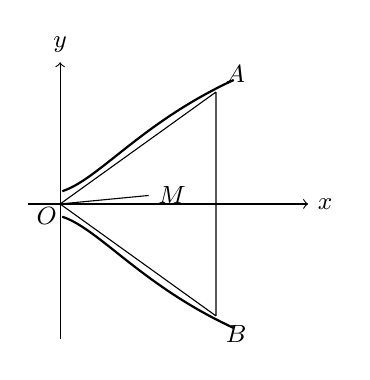
\begin{tikzpicture}[scale=0.9,font=\small]
  \draw[->] (-0.45,0)--(3.5,0) node[right] {$x$};
  \draw[->] (0,-1.9)--(0,2.0) node[above] {$y$};
  \node[below left,inner sep=1pt] at (0,0) {$O$};
  % Schematic right-opening parabola; not a fitted curve.
  \draw[thick] (0.03,0.18) .. controls (0.55,0.35) and (1.15,1.15) .. (2.45,1.75);
  \draw[thick] (0.03,-0.18) .. controls (0.55,-0.35) and (1.15,-1.15) .. (2.45,-1.75);
  \coordinate (A) at (2.2,1.58); \coordinate (B) at (2.2,-1.58);
  \coordinate (M) at (1.25,0.12);
  \draw (0,0)--(A) (0,0)--(B) (A)--(B) (0,0)--(M);
  \node[above right] at (A) {$A$}; \node[below right] at (B) {$B$};
  \node[right] at (M) {$M$};
\end{tikzpicture}
